\documentclass[10pt]{article}
\usepackage[utf8]{inputenc}
\usepackage[T1]{fontenc}
\usepackage{amsmath}
\usepackage{amsfonts}
\usepackage{amssymb}
\usepackage[version=4]{mhchem}
\usepackage{stmaryrd}
\usepackage{graphicx}
\usepackage[export]{adjustbox}
\graphicspath{ {./images/} }
\usepackage{caption}

\begin{document}

\section*{Data Analysis 1: 'Distance to the Large Magellanic Cloud'}
In 2019 an international collaboration led by Polish astronomers measured, with very high precision and accuracy, the distance to the Large Magellanic Cloud (LMC), a satellite galaxy of the Milky Way. In this way they set the zero point of the extragalactic distance scale, which allowed for a very precise measurement of the Hubble constant. Their method involved measuring the distances to 20 eclipsing binary stars in the LMC, using the concept of the surface brightness $S_{V}$ of a star defined as:

$$
S_{V}=m_{V}+5 \log _{10} \theta
$$

where $m_{V}$ is the magnitude of a star in the optical $V$ band and $\theta$ is the angular diameter of the star on the sky in milliarcseconds (mas).

The quantity $S_{V}$ can be understood as the magnitude of a star with an angular diameter of 1 mas. An empirical relation has been established between $S_{V}$ and the colour index $\left(m_{V}-m_{K}\right)$, where $m_{V}$ and $m_{K}$ are magnitudes in the $V$-band and infrared $K$-band. This is shown in the figure below for giant stars of spectral types G and K .\\
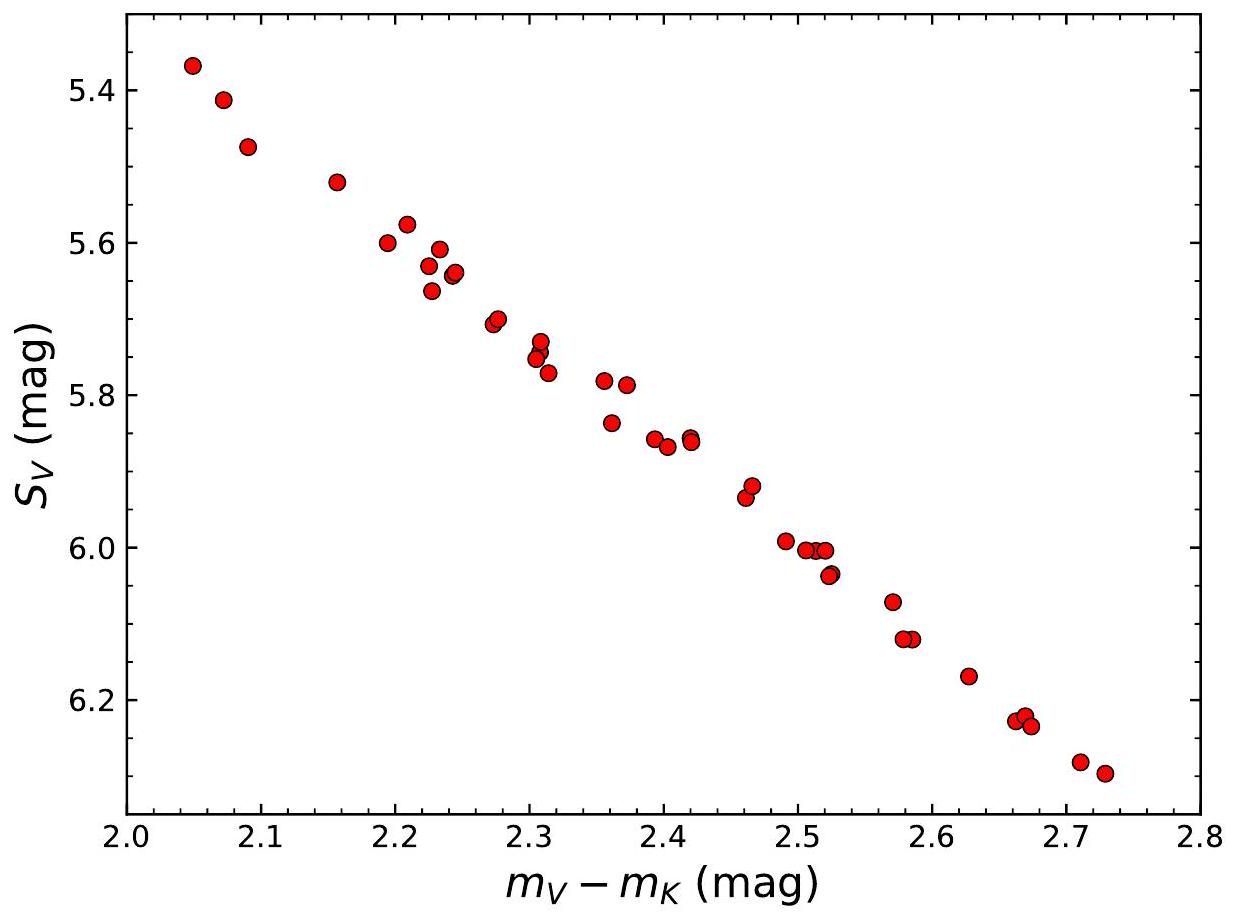
\includegraphics[max width=\textwidth, center]{2025_09_11_2a6858dd99d789184a35g-02}

Using this relation, the distance to an eclipsing binary system can be determined by deriving the physical radii of the components (using photometry and spectroscopy), and comparing these with the angular diameters predicted by the $S_{V}-\left(m_{V}-m_{K}\right)$ relation.\\
The table below gives the parameters of three detached eclipsing binary stars. $R_{1}$ and $R_{2}$ are the radii of each component, $V_{1+2}$ and $K_{1+2}$ are the total brightness in magnitudes of the binary in the $V$ - and $K$-bands, and $L_{2} / L_{1}$ is the luminosity ratio of the components in each band.

\begin{center}
\begin{tabular}{|c|c|c|c|c|c|c|}
\hline
source ID & $\boldsymbol{R}_{\mathbf{1}}\left[\boldsymbol{R}_{\boldsymbol{\odot}}\right]$ & $\boldsymbol{R}_{\mathbf{2}}\left[\boldsymbol{R}_{\boldsymbol{\Theta}}\right]$ & $\boldsymbol{V}_{\mathbf{1 + 2}}[\mathbf{m a g}]$ & $\boldsymbol{K}_{\mathbf{1 + 2}}[\mathbf{m a g}]$ & $\boldsymbol{L}_{\mathbf{2}} / \boldsymbol{L}_{\mathbf{1}}(\boldsymbol{V})$ & $\boldsymbol{L}_{\mathbf{2}} / \boldsymbol{L}_{\mathbf{1}}(\boldsymbol{K})$ \\
\hline
OGLE LMC-ECL-03160 & 17.03 & 37.42 & 16.73 & 14.10 & 2.80 & 4.23 \\
\hline
OGLE LMC-ECL-10567 & 24.60 & 36.64 & 16.15 & 13.83 & 1.41 & 1.99 \\
\hline
OGLE LMC-ECL-18365 & 37.30 & 15.94 & 16.27 & 14.01 & 0.206 & 0.188 \\
\hline
\end{tabular}
\end{center}

Apply the method outlined above to the three eclipsing binary systems and calculate the distance to the LMC in kiloparsecs. Estimate the total error of the result. Assume that the fitting of the $S_{V}-\left(m_{V}-m_{K}\right)$ relation contributes to a bias of up to $0.8 \%$ in all measurements simultaneously.\\
(Total: 50 points)

Hint: in your calculations keep at least three significant figures and two decimal places. Assume that interstellar extinction is negligible and that the angular size of the LMC is small.

\end{document}